%%%%%%%%%%%%%%%%%%%%%%%%%%%%%%%%%%%%%%%%%%%%%%%%%%%%%%%%%%%%%%%%
% DOCUMENT DEFINITION AND BASIC SETTINGS
%%%%%%%%%%%%%%%%%%%%%%%%%%%%%%%%%%%%%%%%%%%%%%%%%%%%%%%%%%%%%%%%
\documentclass[12pt,a4paper,colorlinks=true,linkcolor=NavyBlue,citecolor=red,urlcolor=NavyBlue]{book}
\usepackage[utf8]{inputenc}
\usepackage[T1]{fontenc}
\usepackage[polish]{babel}         

%%%%%%%%%%%%%%%%%%%%%%%%%%%%%%%%%%%%%%%%%%%%%%%%%%%%%%%%%%%%%%%%
% FONT AND STYLE PACKS
%%%%%%%%%%%%%%%%%%%%%%%%%%%%%%%%%%%%%%%%%%%%%%%%%%%%%%%%%%%%%%%%
\usepackage{mathpazo}             
\usepackage[semibold]{sourcesanspro}
\usepackage{sectsty}
\allsectionsfont{\sffamily} 

%%%%%%%%%%%%%%%%%%%%%%%%%%%%%%%%%%%%%%%%%%%%%%%%%%%%%%%%%%%%%%%%
% COLORS AND GRAPHIC STYLES
%%%%%%%%%%%%%%%%%%%%%%%%%%%%%%%%%%%%%%%%%%%%%%%%%%%%%%%%%%%%%%%%
\usepackage{color}
\definecolor{Valentia}{RGB}{233,78,82}
\definecolor{Titleblue}{RGB}{114,146,162}

%%%%%%%%%%%%%%%%%%%%%%%%%%%%%%%%%%%%%%%%%%%%%%%%%%%%%%%%%%%%%%%%
% LAYOUT AND FORMATTING PACKAGES
%%%%%%%%%%%%%%%%%%%%%%%%%%%%%%%%%%%%%%%%%%%%%%%%%%%%%%%%%%%%%%%%
\usepackage{mdframed}
\usepackage{multirow}
\usepackage{multicol}
\usepackage{tikz}
\usepackage{graphicx}
\usepackage[absolute]{textpos}
\usepackage{colortbl}
\usepackage{array}
\usepackage{geometry}
\usepackage{scrextend}

%%%%%%%%%%%%%%%%%%%%%%%%%%%%%%%%%%%%%%%%%%%%%%%%%%%%%%%%%%%%%%%%
% HEADER AND FOOTER SETTINGS
%%%%%%%%%%%%%%%%%%%%%%%%%%%%%%%%%%%%%%%%%%%%%%%%%%%%%%%%%%%%%%%%
\usepackage{fancyhdr}
\pagestyle{fancy}
\fancyhf{}
\fancyheadoffset{0.005\textwidth}
\fancyhead[LE]{\thepage}
\fancyhead[RE]{\nouppercase\leftmark}
\fancyhead[RO]{\thepage}
\fancyhead[LO]{\nouppercase\rightmark}

%%%%%%%%%%%%%%%%%%%%%%%%%%%%%%%%%%%%%%%%%%%%%%%%%%%%%%%%%%%%%%%%
% HYPERLINKS AND CHAPTER STYLES
%%%%%%%%%%%%%%%%%%%%%%%%%%%%%%%%%%%%%%%%%%%%%%%%%%%%%%%%%%%%%%%%
\usepackage{hyperref}
\usepackage[Sonny]{fncychap}
\usepackage[colorlinks=true, linkcolor=blue, citecolor=red, urlcolor=blue]{hyperref}

%%%%%%%%%%%%%%%%%%%%%%%%%%%%%%%%%%%%%%%%%%%%%%%%%%%%%%%%%%%%%%%%
% BEGINNING OF THE DOCUMENT
%%%%%%%%%%%%%%%%%%%%%%%%%%%%%%%%%%%%%%%%%%%%%%%%%%%%%%%%%%%%%%%%
\begin{document}

%%%%%%%%%%%%%%%%%%%%%%%%%%%%%%%%%%%%%%%%%%%%%%%%%%%%%%%%%%%%%%%%
% TITLE PAGE
%%%%%%%%%%%%%%%%%%%%%%%%%%%%%%%%%%%%%%%%%%%%%%%%%%%%%%%%%%%%%%%%
\begin{titlepage}
\newgeometry{left=2.5cm, bottom=3cm, top=2cm, right=2.5cm}

\tikz[remember picture,overlay] \node[opacity=0.03,inner sep=0pt] at (73.6mm, -124.25mm){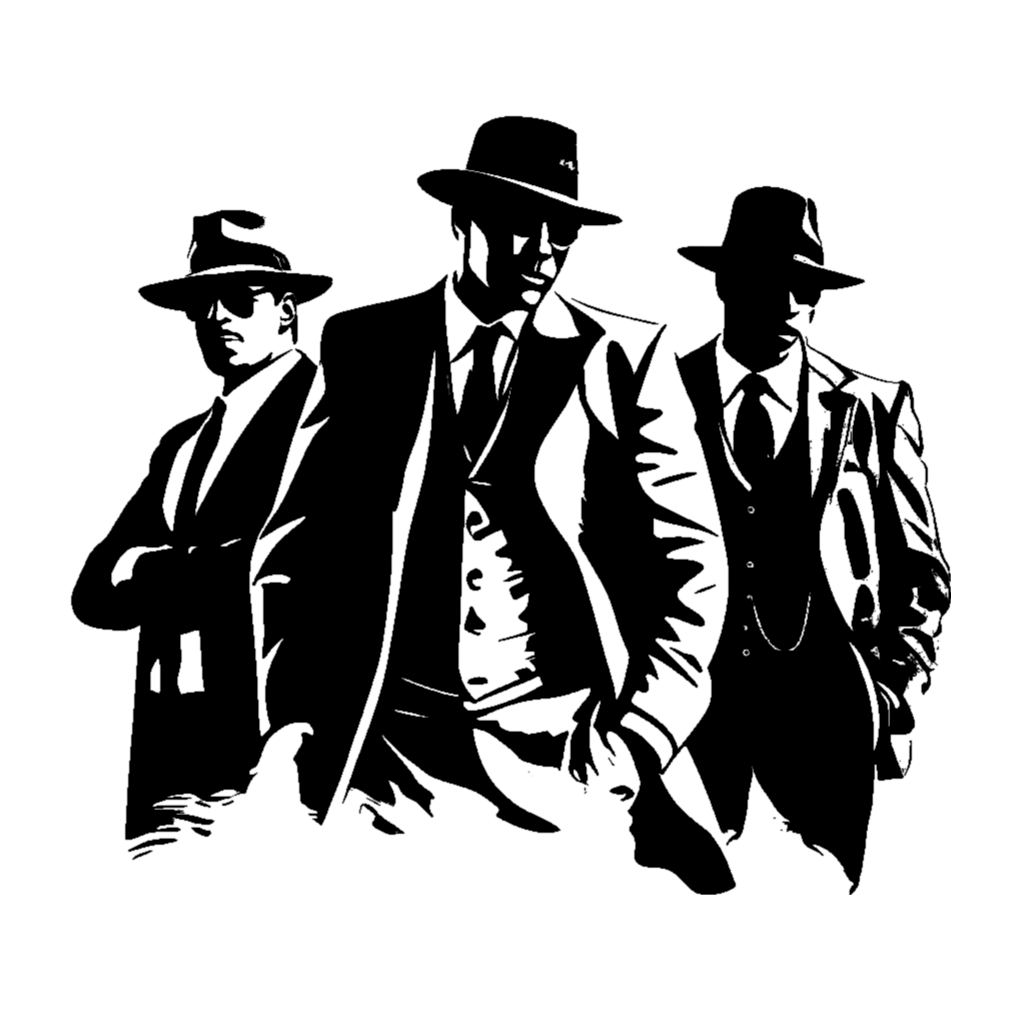
\includegraphics{characters.png}};

\centering
\color{black}
\fontsize{24}{13}\selectfont
\textbf{DOKUMENT PROJEKTU} \\[2mm]
\normalsize
\color{black}
\bigskip
\textbf{Wersja dokumentu: 1.0}\\[1mm]
\bigskip
\textbf{Data utworzenia: 10.06.2025}\\[1mm]
\bigskip
\textbf{Data ostatniej aktualizacji: 10.06.2025}

% Title of the project
\color{black}
\vspace{2cm}
{\fontsize{28}{32} \selectfont \textbf{Gra internetowa}}\\ 
\vspace{0.3cm} 
{\fontsize{45}{32} \selectfont \textbf{Codenames}} 

% Subtitle of the project
\vspace{2cm}
\fontsize{15}{18}\selectfont
\color{black}
\textbf{Dobór metodyki\\}
\bigskip
\vspace{5cm}

% Information about authors
\normalsize
\bigskip
\fontsize{12}{12}\selectfont
\vspace{1.5mm}
\raggedright
\begin{tabular}{ll}
\textbf{Redaktor:} & Adam Chabraszewski \\[6mm]
\textbf{Współautorzy:}
& Zuzanna Nowak \\[2mm]
& Agata Domasik \\[2mm]
& Jakub Walasik \\[6mm]
\textbf{Liczba stron:} & 24 \\[2mm]
\end{tabular}

% Logo
\vspace{\fill}
\begin{center}
    
\includegraphics[scale=0.3]{logo.png} 
\end{center}
\vspace{-15mm}
\end{titlepage}

%%%%%%%%%%%%%%%%%%%%%%%%%%%%%%%%%%%%%%%%%%%%%%%%%%%%%%%%%%%%%%%%
% GEOMETRY SETTINGS FOR THE MAIN BODY OF THE DOCUMENT
%%%%%%%%%%%%%%%%%%%%%%%%%%%%%%%%%%%%%%%%%%%%%%%%%%%%%%%%%%%%%%%%
\newgeometry{top=2cm, bottom=2.5cm, left=2cm, right=2cm}

%%%%%%%%%%%%%%%%%%%%%%%%%%%%%%%%%%%%%%%%%%%%%%%%%%%%%%%%%%%%%%%%
% CONTENT OF THE DOCUMENT
%%%%%%%%%%%%%%%%%%%%%%%%%%%%%%%%%%%%%%%%%%%%%%%%%%%%%%%%%%%%%%%%

%%%%%%%%%%%%%%%%%%%%%%%%%%%%%%%%%%%%%%%%%%%%%%%%%%%%%%%%%%%%%%%%
% TABLE OF CONTENTS
%%%%%%%%%%%%%%%%%%%%%%%%%%%%%%%%%%%%%%%%%%%%%%%%%%%%%%%%%%%%%%%%
\tableofcontents

\chapter{Wprowadzenie - o dokumencie}
\section{Cel dokumentu}
Celem niniejszego dokumentu jest dokonanie analizy projektu informatycznego w kontekście wyboru i dostosowania odpowiedniej metodyki prowadzenia projektu. Analiza oparta jest na ocenach według modelu uproszczonego oraz modelu pełnego, z uwzględnieniem pięciu oraz siedmiu kryteriów oceny. Dokument zawiera również określenie modelu dostarczania produktu końcowego oraz wybór konkretnej metodyki projektowej wraz z propozycją jej adaptacji do specyfiki projektu. 
Celem końcowym jest świadomy wybór i uzasadnienie metodyki zarządzania projektem, która najlepiej wspiera realizację celów projektowych w danych warunkach organizacyjnych, technicznych i zespołowych.

\section{Odbiorcy}

\begin{itemize}
    \item Dr inż. Jakub Miler - prowadzący przedmiot \textit{Realizacja projektu informatycznego},
    \item Dr inż. Katarzyna Łukasiewicz - prowadzący zajęcia projektowe,
    \item Katedra Inżynierii Oprogramowania, \\[2mm] 
Wydział Elektroniki, Telekomunikacji i Informatyki, \\[2mm]  
Politechnika Gdańska,
    \item Członkowie zespołu projektowego:
    \begin{itemize}
        \item[] Zuzanna Nowak, 193165 - kierownik projektu
        \item[] Agata Domasik, 193577
        \item[] Jakub Walasik, s193650
        \item[] Adam Chabraszewski, s193373
    \end{itemize}
\end{itemize}

\clearpage

%%%%%%%%%%%%%%%%%%%%%%%%%%%%%%%%%%%%%%%%%%%%%%%%%%%%%%%%%%%%%%%%
% Chapters
%%%%%%%%%%%%%%%%%%%%%%%%%%%%%%%%%%%%%%%%%%%%%%%%%%%%%%%%%%%%%%%%
\chapter{Charakterystyka projektu}

\section{Opis projektu}
Projekt dotyczy stworzenia gry internetowej \textbf{Codenames}, rozgrywanej w trybie multiplayer z obsługą logowania (OAuth), tworzenia lobby oraz czatu. Gra inspirowana jest popularną grą planszową o tej samej nazwie. Wersja cyfrowa wymaga implementacji mechanik rozgrywki, komunikacji w czasie rzeczywistym (np. przez WebSocket), a także podstawowej logiki serwerowej i interfejsu użytkownika.

\section{Zespół}
Zespół liczy 4 osoby. Część zespołu posiada doświadczenie komercyjne, pozostałe osoby mają doświadczenie akademickie. Komunikacja przebiega sprawnie – zespół wykorzystywał \textit{planning poker} do szacowania zadań oraz pracował w trybie zdalnym. 

\section{Klient i zaangażowanie}
Projekt realizowany był na potrzeby zaliczenia przedmiotu, a klientem pełniącym rolę właściciela produktu był prowadzący zajęcia. Był on regularnie dostępny do udzielania informacji zwrotnej, co umożliwiało iteracyjne podejście do pracy i szybką adaptację do zmian wymagań.

\section{Technologie}
W projekcie zastosowano technologie webowe – w tym React do budowy interfejsu użytkownika, Java Spring jako backend oraz WebSocket do komunikacji czatu w czasie rzeczywistym. Autoryzacja użytkowników odbywa się z wykorzystaniem OAuth2 (Google).

\section{Charakterystyka biznesowa}
Wymagania klienta zmieniały się dynamicznie – szczególnie w obszarach interfejsu użytkownika, UX rozgrywki i logiki działania. Szybkie dostarczanie przyrostów i możliwość natychmiastowego testowania miały kluczowe znaczenie.


\newpage
\thispagestyle{empty}
\null
\newpage

%%%%%%%%%%%%%%%%%%%%%%%%%%%%%%%%%%%%%%%%%%%%%%%%%%%%%%%%%%%%%%%%
% Chapters
%%%%%%%%%%%%%%%%%%%%%%%%%%%%%%%%%%%%%%%%%%%%%%%%%%%%%%%%%%%%%%%%

\chapter{Ocena według modelu uproszczonego – 5 kryteriów}

\section{Ocena modelu}

W celu określenia najlepiej dopasowanej metodyki do realizacji projektu, oceniliśmy nasz projekt w pięciu kategoriach zgodnie z modelem uproszczonym:

\begin{itemize}
  \item \textbf{Rozmiar:} średni – projekt był realizowany przez zespół 4-osobowy w ciągu jednego semestru. Liczba funkcjonalności była umiarkowana, ale wymagała integracji wielu technologii.
  
  \item \textbf{Krytyczność:} niska – projekt nie był przeznaczony do zastosowań krytycznych. Nie było konieczności zapewnienia wysokiej niezawodności czy bezpieczeństwa danych.
  
  \item \textbf{Dynamika:} wysoka – wymagania projektowe zmieniały się dynamicznie, głównie ze względu na iteracyjny kontakt z klientem i zmieniające się oczekiwania względem UX.
  
  \item \textbf{Osoby:} doświadczone technicznie, ale niekomercyjnie jako zespół – mimo że część zespołu miała doświadczenie komercyjne, zespół jako całość nie pracował wcześniej razem. Uzasadnia to potrzebę elastycznego podejścia.
  
  \item \textbf{Kultura organizacyjna:} otwarta i oparta na zaufaniu – zespół miał dużą autonomię i wykorzystywał praktyki zwinne (planowanie iteracyjne, szybka komunikacja, retrospekcje).
\end{itemize}

\noindent
Na podstawie powyższych ocen, projekt lepiej wpisuje się w metodyki \textbf{zwinne (Agile)}, takie jak Scrum lub Kanban. Dynamiczne wymagania, otwarta komunikacja i zmieniające się priorytety lepiej wspierają podejście iteracyjne niż kaskadowe.

\begin{figure}[H]
  \centering
  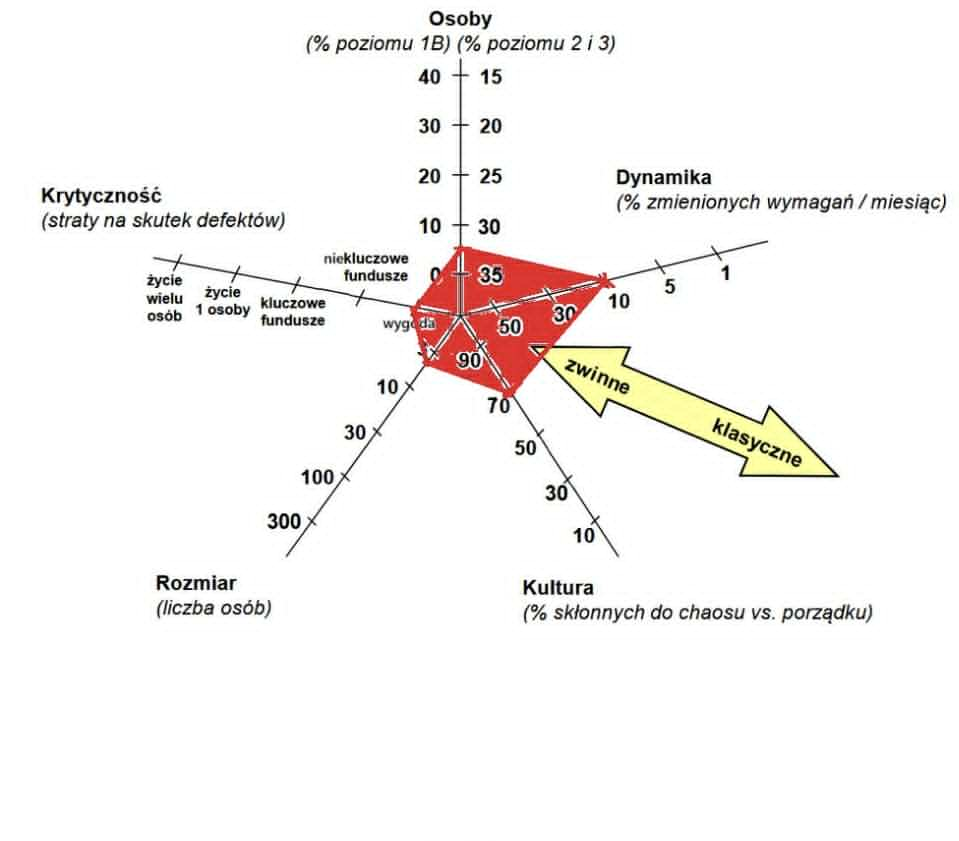
\includegraphics[width=0.8\textwidth]{ocena_modelu.jpeg}
  \caption{Ocena projektu w 5 kategoriach – model uproszczony}
\end{figure}


\newpage
\thispagestyle{empty}
\null
\newpage

%%%%%%%%%%%%%%%%%%%%%%%%%%%%%%%%%%%%%%%%%%%%%%%%%%%%%%%%%%%%%%%%
% Chapters
%%%%%%%%%%%%%%%%%%%%%%%%%%%%%%%%%%%%%%%%%%%%%%%%%%%%%%%%%%%%%%%%

\newpage
\thispagestyle{empty}
\null
\newpage

%%%%%%%%%%%%%%%%%%%%%%%%%%%%%%%%%%%%%%%%%%%%%%%%%%%%%%%%%%%%%%%%
% Chapters
%%%%%%%%%%%%%%%%%%%%%%%%%%%%%%%%%%%%%%%%%%%%%%%%%%%%%%%%%%%%%%%%

\chapter{Ocena według zaadaptowanego modelu pełnego – 7 kryteriów}

\section{Ocena}

Na podstawie rozszerzonego modelu oceny projektów, projekt został przeanalizowany w 4 obszarach, obejmujących 7 kryteriów. Dla każdego kryterium określono charakterystykę projektu oraz dopasowanie do „własnego podwórka” konkretnego typu metodyki.

\section{Zastosowanie}

\begin{itemize}
  \item \textbf{Główne cele:} celem projektu było stworzenie działającej aplikacji zgodnej z wymaganiami klienta końcowego. Projekt miał charakter eksploracyjno-edukacyjny, co sprzyja stosowaniu metodyk zwinnych (Agile), gdzie istotna jest iteracja i ciągłe dostosowanie do potrzeb.
  
  \item \textbf{Środowisko:} środowisko było umiarkowanie złożone, z wieloma zmiennymi – zarówno technicznymi (integracja różnych narzędzi), jak i organizacyjnymi (terminy, konsultacje z prowadzącym). Warunki te sugerują lepsze dopasowanie do podejścia zwinnego.
\end{itemize}

\section{Zarządzanie}

\begin{itemize}
  \item \textbf{Komunikacja:} zespół korzystał z codziennej asynchronicznej komunikacji (czat), tygodniowych spotkań synchronizacyjnych i tablicy zadań. Taki styl pracy wspiera metodyki zwinne, gdzie komunikacja jest kluczowa i ciągła.
\end{itemize}

\section{Techniczne}

\begin{itemize}
  \item \textbf{Wymagania:} wymagania były początkowo ogólne, a następnie doprecyzowywane w trakcie prac. Zmienność i niepełność wymagań preferuje podejście iteracyjne i adaptacyjne – typowe dla Agile.
  
  \item \textbf{Wytwarzanie:} projekt był rozwijany iteracyjnie, w krótkich sprintach, z częstym testowaniem i prezentowaniem postępów. Brak był ścisłego planu całego procesu na początku, co znów wskazuje na Agile jako lepsze dopasowanie.
\end{itemize}

\section{Osoby}

\begin{itemize}
  \item \textbf{Klient:} klient (prowadzący) był dostępny cyklicznie, przekazywał informację zwrotną i modyfikował oczekiwania. Współpraca i zaangażowanie klienta wskazują na zwinne podejście.
  
  \item \textbf{Kultura:} zespół pracował w atmosferze wzajemnego zaufania, z dużą autonomią i elastycznością. Kultura taka jest typowa dla metodyk zwinnych, gdzie samodzielność i inicjatywa członków zespołu są wysoko cenione.
\end{itemize}

\noindent
\textbf{Podsumowanie:} Wszystkie analizowane kryteria wskazują na lepsze dopasowanie naszego projektu do metodyk \textbf{zwinnych (Agile)}. Projekt cechował się zmiennością, iteracyjnym wytwarzaniem, częstą komunikacją i aktywnym udziałem klienta. Model pełny tylko potwierdza wcześniejszą ocenę opartą na modelu uproszczonym.


\newpage
\thispagestyle{empty}
\null
\newpage

%%%%%%%%%%%%%%%%%%%%%%%%%%%%%%%%%%%%%%%%%%%%%%%%%%%%%%%%%%%%%%%%
% Chapters
%%%%%%%%%%%%%%%%%%%%%%%%%%%%%%%%%%%%%%%%%%%%%%%%%%%%%%%%%%%%%%%%

\chapter{Model dostarczania produktu końcowego projektu}

\section{Model}

W naszym projekcie zastosowano \textbf{model przyrostowy} dostarczania produktu końcowego. Oznacza to, że produkt był rozwijany i udostępniany etapami, w kolejnych wersjach zawierających coraz bardziej rozbudowane funkcjonalności.

Taki model dostarczania pozwalał na:
\begin{itemize}
  \item \textbf{Stopniową realizację wymagań} – najpierw implementowano podstawowe funkcje, a następnie bardziej zaawansowane moduły.
  \item \textbf{Regularne testowanie} – każda kolejna wersja była testowana przez członków zespołu, a błędy były usuwane na bieżąco.
  \item \textbf{Elastyczne reagowanie na zmiany} – możliwe było modyfikowanie planu działania w zależności od postępów i informacji zwrotnej.
  \item \textbf{Częstą prezentację postępów klientowi} – po każdym przyroście klient mógł ocenić efekty i zaproponować zmiany.
\end{itemize}

Model ten doskonale współgra z \textbf{metodykami zwinnymi (Agile)}, które zakładają iteracyjne podejście do wytwarzania oprogramowania, częste dostarczanie działających fragmentów systemu oraz ścisłą współpracę z klientem.

\noindent
\textbf{Podsumowanie:} Wybór modelu przyrostowego był świadomą decyzją wynikającą z charakteru projektu – zmienne wymagania, ograniczony czas oraz chęć szybkiego testowania rozwiązań. Takie podejście minimalizowało ryzyko i zwiększało jakość końcowego produktu.


\newpage
\thispagestyle{empty}
\null
\newpage

%%%%%%%%%%%%%%%%%%%%%%%%%%%%%%%%%%%%%%%%%%%%%%%%%%%%%%%%%%%%%%%%
% Chapters
%%%%%%%%%%%%%%%%%%%%%%%%%%%%%%%%%%%%%%%%%%%%%%%%%%%%%%%%%%%%%%%%

\chapter{Metodyka i jej adaptacja}

\section{Metodyka i jej adaptacja}

Na podstawie analiz przeprowadzonych w punktach 2, 3 i 4, dla realizowanego projektu jako najbardziej odpowiednią wskazano \textbf{metodykę zwinną}, a dokładniej \textbf{Scrum}. Decyzja ta została oparta na następujących przesłankach:

\begin{itemize}
  \item \textbf{Kryteria modelu uproszczonego (punkt 2)} wskazują na średnią wielkość projektu, umiarkowaną krytyczność, dynamiczne wymagania, mały zespół oraz kulturę pracy otwartą na zmiany — co sprzyja metodykom zwinnym.
  \item \textbf{Ocena według modelu pełnego (punkt 3)} również wykazała zgodność większości kryteriów z metodykami zwinnymi: zmienne wymagania, komunikacja bezpośrednia, klient blisko zespołu i kultura wspierająca współpracę.
  \item \textbf{Model dostarczania produktu (punkt 4)} to model przyrostowy — idealnie pasujący do iteracyjnego charakteru Scrum.
\end{itemize}

\section{Wybór konkretnej metodyki}

Z uwagi na powyższe, jako bazową metodykę wybrano \textbf{Scrum}, ponieważ:
\begin{itemize}
  \item Umożliwia iteracyjne planowanie i realizację.
  \item Zakłada częste przeglądy i dostarczanie działających przyrostów produktu.
  \item Wymusza ścisłą komunikację wewnątrz zespołu i z interesariuszami.
  \item Dobrze sprawdza się w małych zespołach.
\end{itemize}

\section{Niedopasowania i adaptacje}

Pomimo ogólnego dopasowania Scrum do projektu, zidentyfikowano kilka elementów projektu, które wymagają adaptacji metodyki:

\subsection*{1. Brak pełnoetatowego właściciela produktu (Product Ownera)}
\textbf{Problem:} Klient nie był dostępny codziennie do współpracy w roli Product Ownera.\\
\textbf{Adaptacja:} Rolę PO przejął jeden z członków zespołu, który pełnił funkcję pośrednika i koordynował zbieranie wymagań oraz zatwierdzanie kolejnych wersji.\\
\textbf{Uzasadnienie:} Umożliwiło to utrzymanie jednolitego kanału komunikacji, mimo ograniczonego dostępu do klienta.

\subsection*{2. Zespół o niepełnym przekroju kompetencji}
\textbf{Problem:} Brak dedykowanego testera i UX designera.\\
\textbf{Adaptacja:} Rozdzielenie tych ról w zespole między programistów — w każdym sprincie część zespołu przeznaczała czas na testowanie i projektowanie interfejsów.\\
\textbf{Uzasadnienie:} Pozwoliło na zachowanie wysokiej jakości mimo braków personalnych.

\subsection*{3. Zbyt krótki czas trwania projektu na pełne wdrożenie Scrum}
\textbf{Problem:} Czas trwania projektu (kilka tygodni) był zbyt krótki na pełne wdrożenie wszystkich ról, ceremonii i artefaktów Scrum.\\
\textbf{Adaptacja:} Zredukowano liczbę spotkań — zamiast codziennych Daily Scrumów, odbywały się one 2–3 razy w tygodniu.\\
\textbf{Uzasadnienie:} Zachowano regularną synchronizację, nie obciążając zespołu nadmiarem formalności.

\subsection*{4. Wysoka zmienność wymagań także w środku sprintu}
\textbf{Problem:} Pojawiały się istotne zmiany w wymaganiach również w trakcie trwających sprintów.\\
\textbf{Adaptacja:} Wprowadzono możliwość częściowego przerywania sprintu (po zatwierdzeniu przez zespół), by włączyć nowe wymagania.\\
\textbf{Uzasadnienie:} Zespół nie tracił elastyczności i mógł reagować na realne potrzeby klienta.

\section{Podsumowanie}

Wybrana metodyka bazowa — \textbf{Scrum} — została zaadaptowana do warunków projektu poprzez zmodyfikowanie ról, częstotliwości spotkań oraz podejścia do zmian w backlogu. Dzięki temu możliwe było zachowanie głównych wartości metodyki zwinnej, jednocześnie dostosowując ją do realiów projektu.


\newpage
\thispagestyle{empty}
\null
\newpage

%%%%%%%%%%%%%%%%%%%%%%%%%%%%%%%%%%%%%%%%%%%%%%%%%%%%%%%%%%%%%%%%
% Chapters
%%%%%%%%%%%%%%%%%%%%%%%%%%%%%%%%%%%%%%%%%%%%%%%%%%%%%%%%%%%%%%%%

%%%%%%%%%%%%%%%%%%%%%%%%%%%%%%%%%%%%%%%%%%%%%%%%%%%%%%%%%%%%%%%%
% END PAGE
%%%%%%%%%%%%%%%%%%%%%%%%%%%%%%%%%%%%%%%%%%%%%%%%%%%%%%%%%%%%%%%%
\newpage
\thispagestyle{empty}
\tikz[remember picture,overlay] \node[opacity=0.03,inner sep=0pt] at (73.6mm, -124.25mm){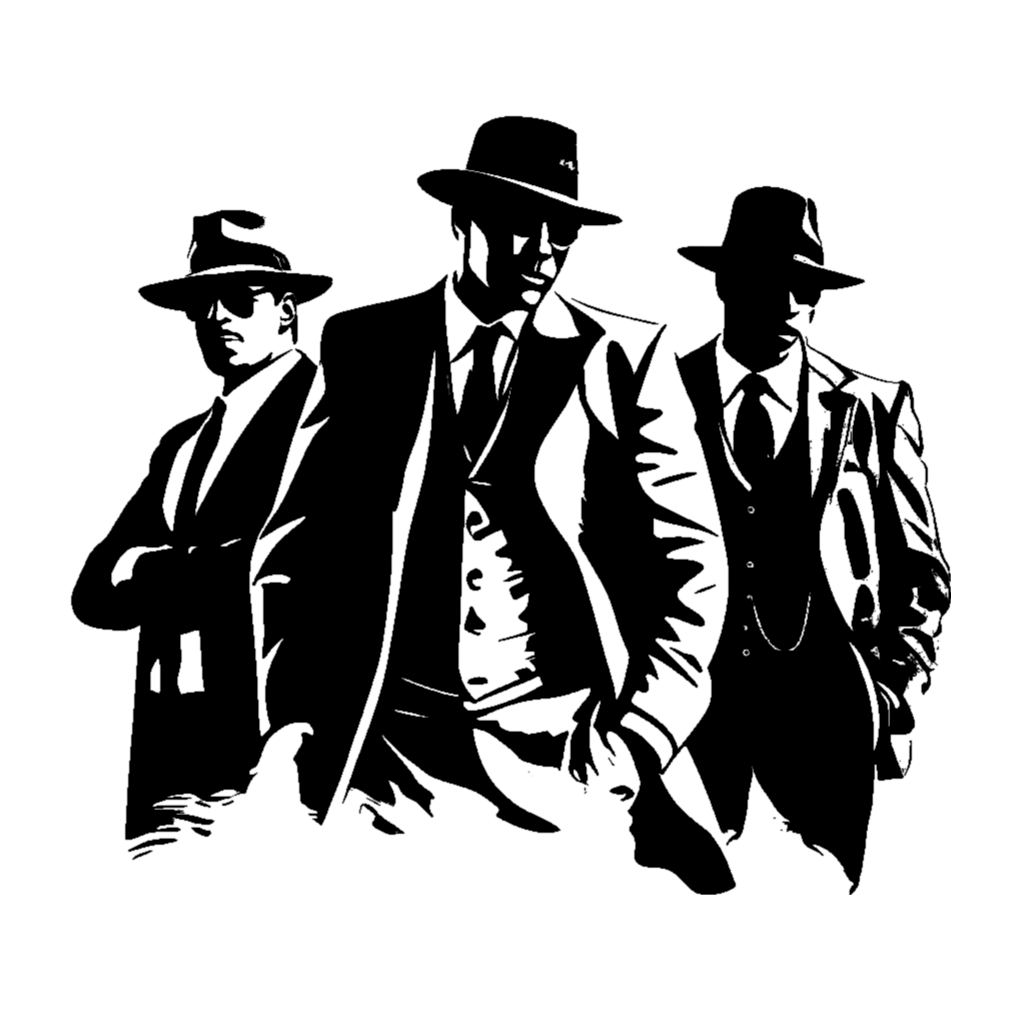
\includegraphics{characters.png}};
\begin{center}
    \vspace*{\fill}
    
\includegraphics[width=0.3\textwidth]{logo.png} 
    \vspace*{\fill}
\end{center}

%%%%%%%%%%%%%%%%%%%%%%%%%%%%%%%%%%%%%%%%%%%%%%%%%%%%%%%%%%%%%%%%
% END OF DOCUMENT
%%%%%%%%%%%%%%%%%%%%%%%%%%%%%%%%%%%%%%%%%%%%%%%%%%%%%%%%%%%%%%%%
\end{document}